\documentclass[letterpaper]{article}
\usepackage{amsmath}
\usepackage{hyperref}
\usepackage{booktabs}
\usepackage{longtable}
\usepackage{graphicx}
%\usepackage{tabularx}

%opening
\title{A note on the minimum number of tests required for sample
	pooling to detect COVID-19 infection}
\author{Robert Jacobson <RobertJacobson@acm.org>}

%\newcommand{\min}[1]{\operatorname{min}{(#1)}}
%\DeclareMathOperator{\min}{min}
%\DeclareMathOperator{\max}{max}

\begin{document}

\maketitle

\begin{abstract}
A variety of authors have investigated the benefits of sample pooling to
test populations for COVID-19 infection. Of primary interest is reducing
the consumption of testing resources, which are a scarce resource during
the COVID-19 pandemic, and the accuracy and efficiency of estimating the
number of infected individuals. This note discusses the limitations
imposed by mathematics on the reduction in number of tests needed to be
performed using this testing method and bounds on the number of infected
individuals in terms of the number of infected pools. Other limitations
related to testing supplies (consumption of pipettes, conical tubes,
etc.), equipment availability, protocol complexity, and so forth are not
discussed. The test for infection is assumed to be 100\% effective and
100\% sensitive.
\end{abstract}

\section{The need for understanding sample pooling}
A variety of authors have investigated the benefits of sample pooling to
test populations for COVID-19 infection. Of primary interest is reducing
the consumption of testing resources, which are a scarce resource during
the COVID-19 pandemic, and the accuracy and efficiency of estimating the
number of infected individuals. This note discusses the limitations
imposed by mathematics on the reduction in number of tests needed to be
performed using this testing method and bounds on the number of infected
individuals in terms of the number of infected pools. Other limitations
related to testing supplies (consumption of pipettes, conical tubes,
etc.), equipment availability, protocol complexity, and so forth are not
discussed. The test for infection is assumed to be 100\% effective and
100\% sensitive.

\section{Sample pooling versus naive sample testing}
\label{sample-pooling-versus-naive-sample-testing}

In naive sample testing, individuals in a population are tested for
infection by taking a sample from every individual and testing each
sample in isolation. In a population of $N$ individuals, naive sample
testing requires $N$ tests.

In (one-dimensional) sample pooling, samples from multiple individuals
are combined into a single pool, and the pool is tested once. A negative
result indicates that no individual in the pool is infected. We call
such a pool a \emph{negative pool}. A positive result indicates that at
least one individual in the pool is infected. We call such a pool a
\emph{positive pool}. In the event of a positive result, the individuals
in the pool must be retested individually to determine which individuals
in the pool are infected. Variations on this method are considered.

The word sample is used in a biological sense, referring to a fluid or
tissue sample from an individual that will be tested for infection. Both
sample pooling and naive sample testing use samples from every
individual in the population. These testing methods should not be
confused with random sampling, which only takes samples from a subset of
the population.

\hypertarget{one-dimensional-sample-pooling}{%
\section{One-dimensional sample pooling}
\label{one-dimensional-sample-pooling}}

In one-dimensional sample pooling, the population of $N$ individuals
is divided into $g:=N/n$ groups of size $n$. The figure below
illustrates a typical qPCR well plate using one-dimensional sample
pooling with $N=96$ and $n=8$, giving $g=12$. Let $i$ be the
number of infected individuals in the population, denoted by red
circles. In this example, $i=3$. The right margin and row background
color indicate the outcome of combining the individuals in the pool (by
row) and testing the pool. In this example, three pools test positive,
because each of the three pools includes an infected individual.


\begin{figure}
	\centering
	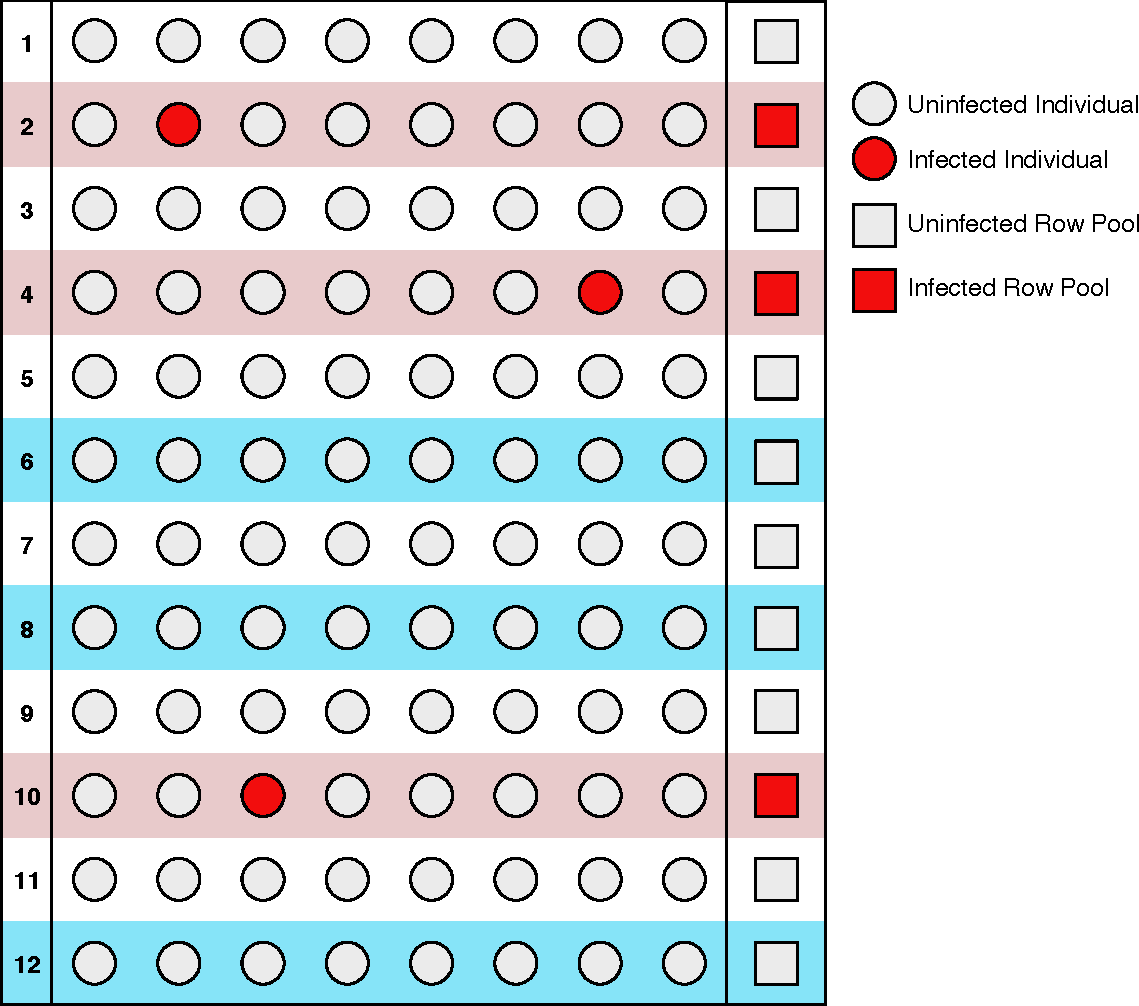
\includegraphics[width=0.8\textwidth]{Fig1DimPooling.pdf}
	\caption{One-dimensional sample pooling.}
\end{figure}


One test is used per pool. In this example, it takes 12 tests to test
all 12 pools. Each individual in the positive pools are tested in
isolation to identify which individuals are infected. The total number
of tests performed is $12 + 3\times 8 = 36$ tests, compared to 96
tests using naive sample testing.

Observe that naive sample testing is equivalent to the degenerate sample
pooling cases of $n=N$ ($g=1$) and $n=1$ ($g=N$). We therefore
require that $1<n<N$ (equivalently that $1<g<N$).

\hypertarget{bounds-on-the-number-of-required-tests-for-one-dimensional-sample-pooling}{%
\subsection{Bounds on the number of required tests for one-dimensional sample pooling}
\label{bounds-on-the-number-of-required-tests-for-one-dimensional-sample-pooling}}

In general, the number of tests required by one-dimensional sample
pooling is $T = g + kn$, where $k$ is the number of distinct pools
containing infected individuals. The largest $k$ can be is
$\text{min}(i, g)$. Thus, $T_{\text{max}}=g + \text{min}(i,g)n$. When
$i\leq g$, then $T_{\text{max}}=g + in$. Likewise, the smallest
$k$ can be is $0$, corresponding to no infections, so
$T_{\text{min}}=g$. If $i\ll g$ and the individuals are distributed
at random, then $k=i$ with high probability. In particular,

\[Pr(k=i)=\frac{g-1}{g}\cdot \frac{g-2}{g}\cdots \frac{g-i+1}{g} = \frac{g!}{g^{i}(g-i)!}.\]


\begin{figure}
	\centering
	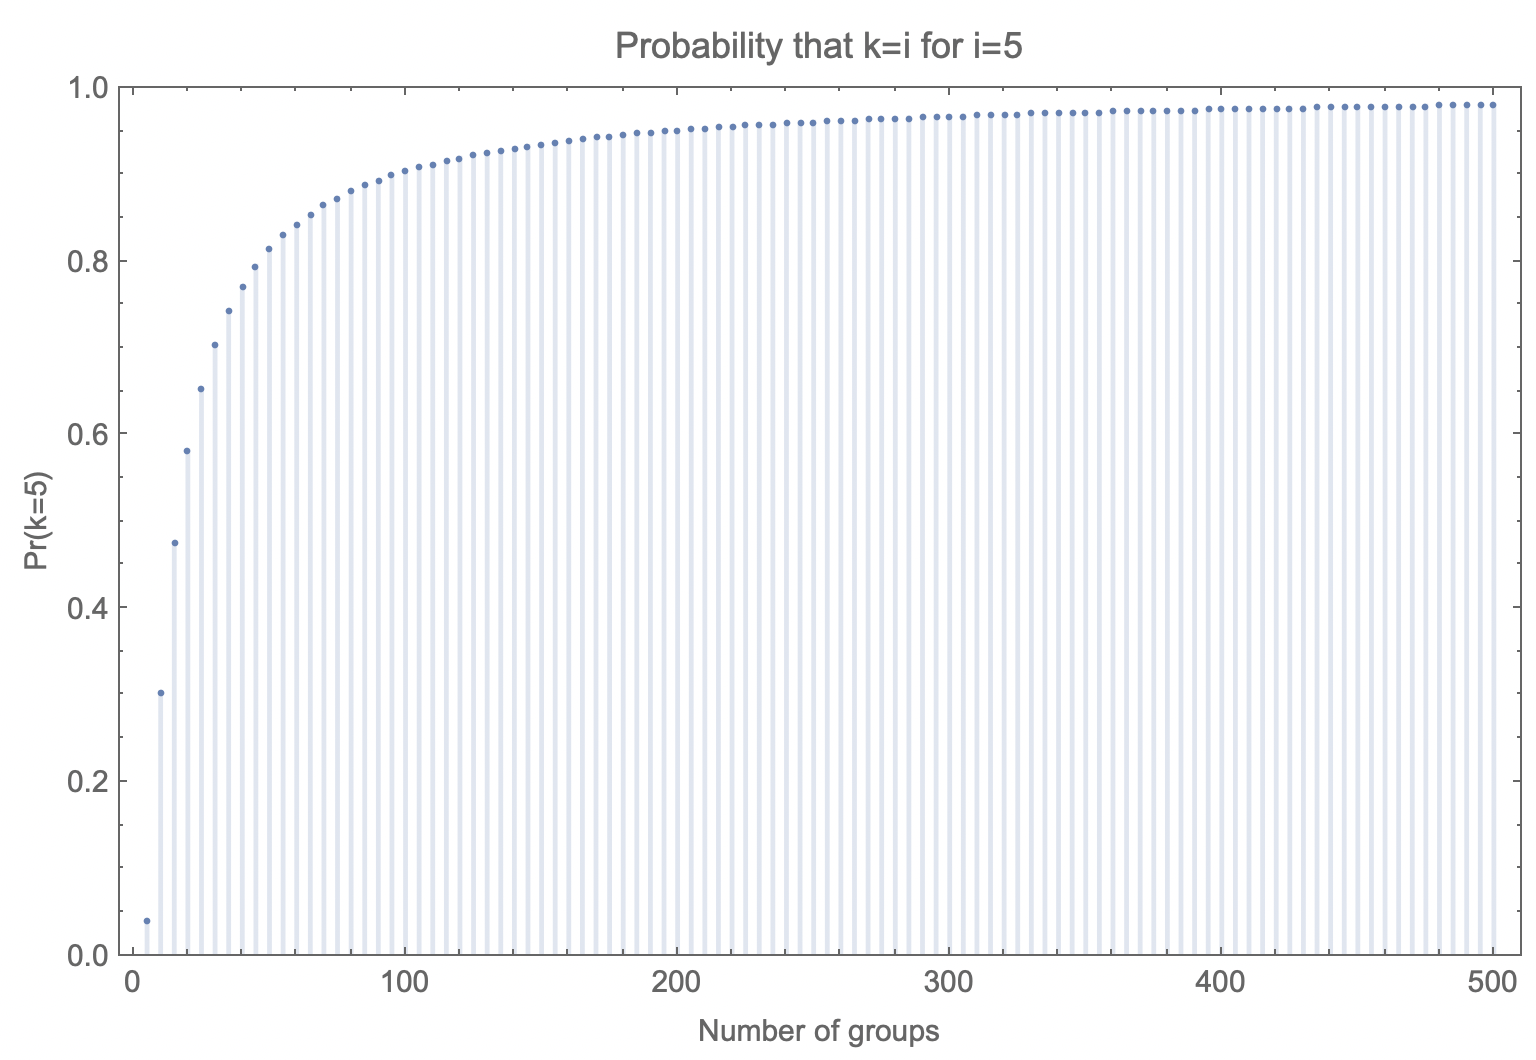
\includegraphics[width=0.8\textwidth]{Prki.png}
	\caption{The probability that no two infected individuals share a
		pool increases as the number of pools increases relative to the number
		of infected individuals. In this graph the number of infected
		individuals is fixed at $i=5$.}
\end{figure}

The real distribution of people infected with COVID-19 is not random,
and Pr$(k=i)$ should not be assumed to follow this formula.

\hypertarget{d-dimensional-sample-pooling}{%
\section{$d$-dimensional sample pooling}
\label{d-dimensional-sample-pooling}}

One-dimensional sample pooling can be improved by simultaneously pooling
the columns as well as the rows. We expand on the previous example in figure~\ref{fig2dimpooling}.


\begin{figure}
	\centering
	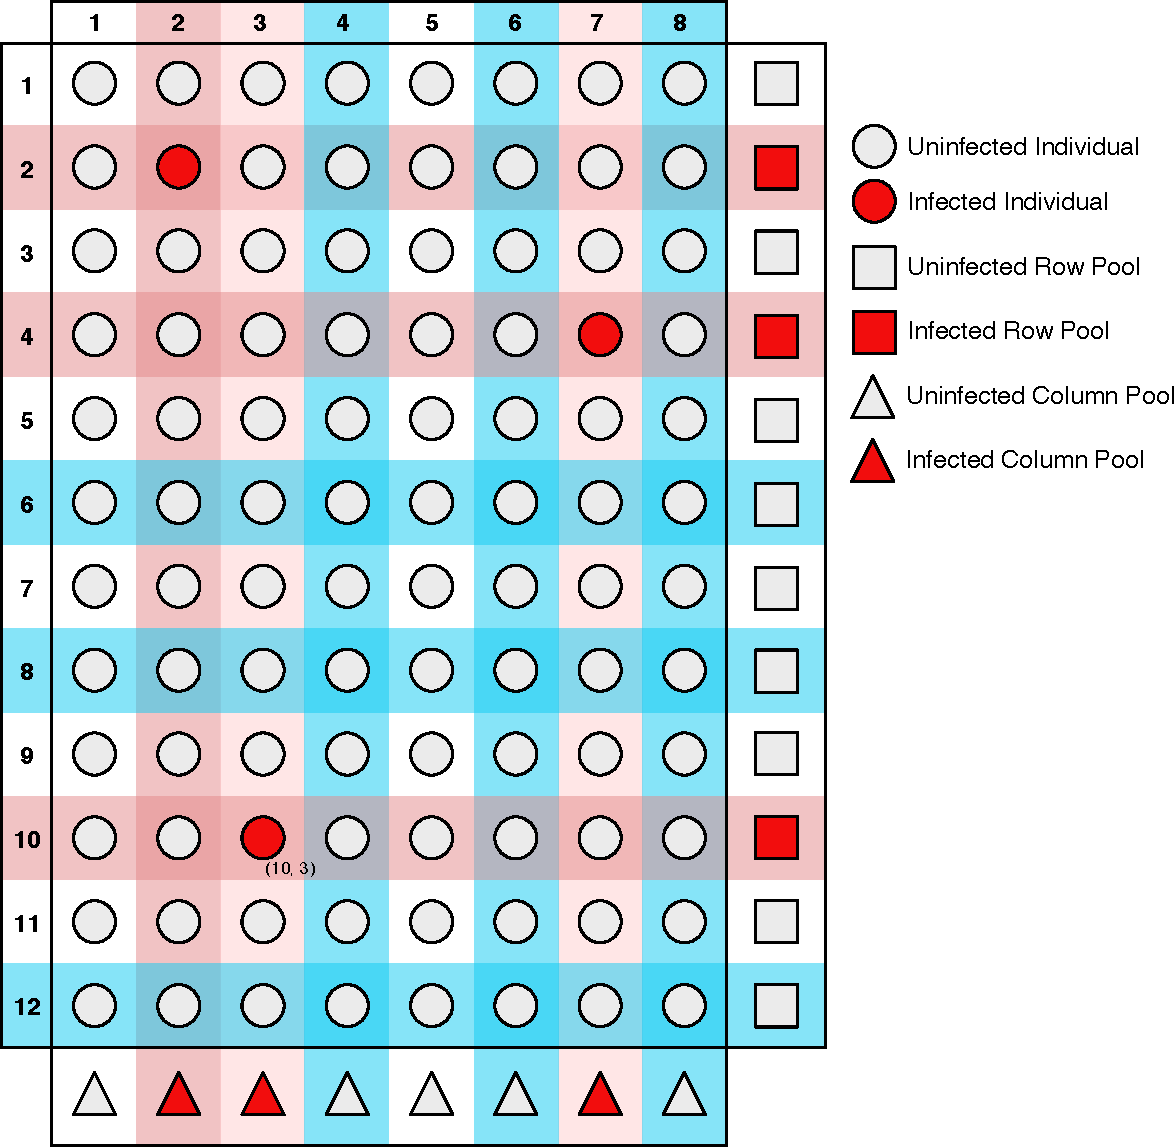
\includegraphics[width=0.8\textwidth]{Fig2DimPooling}
	\caption{Two-dimensional sample pooling.}
	\label{fig2dimpooling}
\end{figure}

An infected individual can only exist at the intersection of a positive
row pool and a positive column pool. However, not every intersection of
a positive row pool and a positive column pool need be an infected
individual. For example, using row-major notation, we see an infected
individual at position $(10, 3)$ but not at position $(10, 2)$. The
benefit is that fewer individuals need to be retested as compared to
one-dimensional sample pooling. In this example, two-dimensional sample
pooling requires $12+8+3^2 = 29$ tests, the maximum possible number
required with this method.

This method can be generalized to $d$-dimensions by indexing each
sample with the set
\[
\{1, 2, 3, \ldots, g_1\}\times \{1, 2, 3, \ldots, g_2\}\times \{1, 2, 3, \ldots, g_3\}\times \cdots \times \{1, 2, 3, \ldots, g_d\},
\]
for positive integers $g_j$ with $1<g_j<N$ and
$\prod_{j=1}^d g_j = g_1\cdot g_2\cdot g_3 \cdots g_d = N$.
The sample pools are the $(d-1)$-dimensional hyperplanes formed by
fixing the value in one coordinate and allowing the other coordinates to
vary. The individuals requiring retesting are those corresponding to the
set of points at the intersection of exactly $d$ positive sample pools
(hyperplanes).

\begin{figure}
\centering
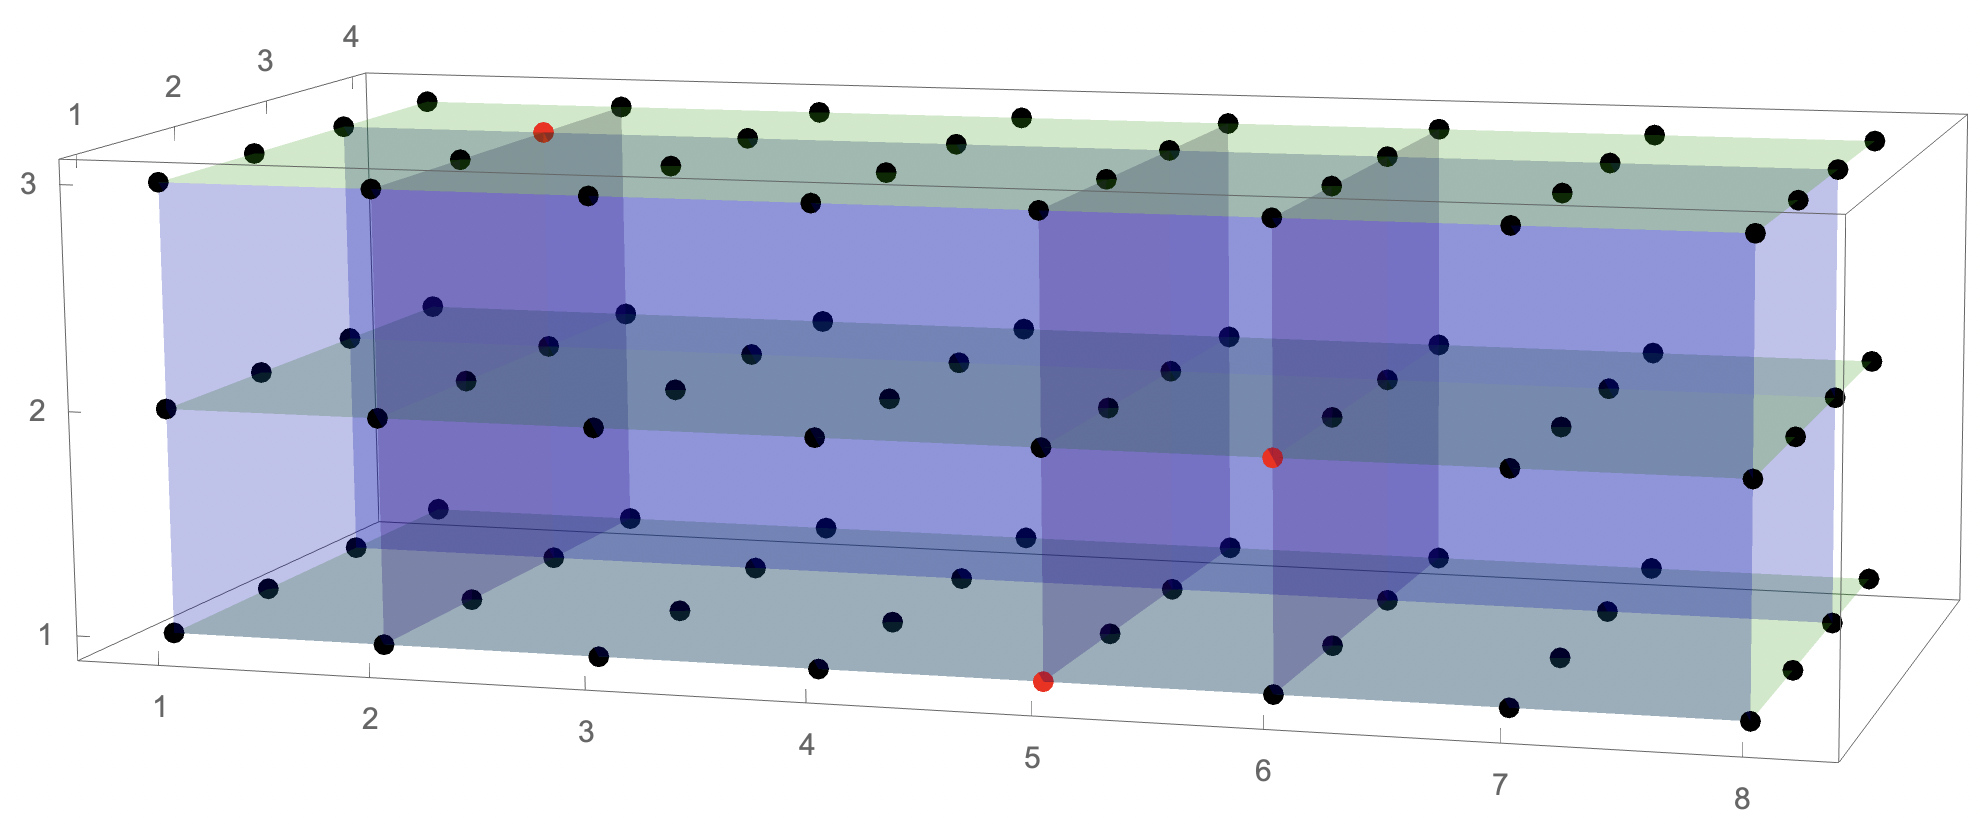
\includegraphics[width=0.8\textwidth]{Fig3DimPooling.png}
\caption{A three-dimensional representation of the previous
	examples. There are 18 points at the intersection of three positive
	pools but only three infected individuals.}
\end{figure}


\hypertarget{a-minor-refinement}{%
\subsection{A minor refinement}\label{a-minor-refinement}}

Instead of testing pools along different dimensions in parallel, testing
along dimensions in sequence and removing every negative pool as it is
discovered reduces the size of pools along dimensions not yet tested.
This does not reduce the number of tests required, as any negative
individual will not lie at the intersection of $d$ pools and hence
will not be in the set of individuals needing to be retested. However,
smaller pool sizes are preferable under more realistic assumptions on
the test and when the conservation of other resources are considered.

\hypertarget{bounds-on-the-number-of-required-tests-for-n-dimensional-sample-pooling}{%
\section{Bounds on the number of required tests for $n$-dimensional sample pooling}
\label{bounds-on-the-number-of-required-tests-for-n-dimensional-sample-pooling}
}

The number of tests required by $d$-dimensional sample pooling is 
\[
T = g_1+g_2+g_3+\cdots + g_d + k_1\cdot k_2 \cdot k_3
\cdots k\_d = \sum_{j=1}^d g_j + \prod_{j=1}^d k_j,
\]
where $k_j$ is the number of distinct positive pools with constant
$j^{\text{th}}$ coordinate for each value of $j$. The series
represents the total number of pools along all dimensions, all of which
must be tested when $i>0$, and is a constant chosen during testing
protocol design. The second term represents the number of retests that
are required to identify which individuals are infected. Clearly the
second term is maximized when either no two positive points lie in the
same pool or, if there are too many infected individuals for that to
happen, when every pool is positive. Thus, the maximum value of $k_j$
is min$(i, g_j)$, and
\[
T_{\text{max}}=\sum_{j=1}^d g_j + \prod_{j=1}^d \text{min}(i, g_j).
\]
Observe that if $i<g_j$ for all $j$, then
\[
T_{\text{max}}=\sum_{j=1}^d g_j + i^d.
\] 
If every individual is infected, then
\[
T_{\text{max}}=\sum_{j=1}^d g_j + \prod_{j=1}^d g_j = \sum_{j=1}^d g_j + N > N.
\]
Sample pooling is therefore worse than naive sample testing when the
number of infected individuals is close to $N$. On the other hand,
there are no infected individuals if and only if there are no positive
pools along any single dimension. If dimensions are tested in order from
smallest to largest, the absence of infected individuals is detectable
after only $\min_j g_j$ tests. Thus, sample pooling gives the
greatest benefit when the number of infected individuals is small.

\hypertarget{reducing-the-number-of-tests-further}{%
\section{Reducing the number of tests further}
\label{reducing-the-number-of-tests-further}}

Consider the example of two-dimensional sample pooling illustrated
in~\ref{fig:shortcut}. The red circles represent infected individuals. 
After testing the pools, represented by the squares and triangles, 
every pool is positive.


\begin{figure}
	\centering
	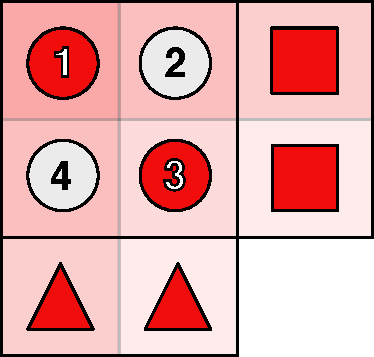
\includegraphics[width=0.3\textwidth]{Shortcut}
	\caption{The pools, represented by the squares and triangles, are
		all positive, whereas there are only two infected individuals.}
	\label{fig:shortcut}
\end{figure}

The retest set is the set of circles lying at the intersection of a
positive row and positive column, which is every circle. The minimum
number of infected individuals needed to have both row pools be positive
is two, one for each row. Similarly, there must be at least two infected
individuals to have two column pools be positive. Without retesting, we
cannot determine whether any particular individual is infected. The
naive approach is to test them all, which requires four tests. Suppose,
however, that we happen to test Circle 2 first, resulting in a negative
outcome, and then Circle 3, giving another negative outcome. We would
then know two particular circles of the four are negative and that there
must be at least two positive circles. We conclude, therefore, that the
remaining two circles must be positive without having to test them.



\begin{figure}
	\centering
	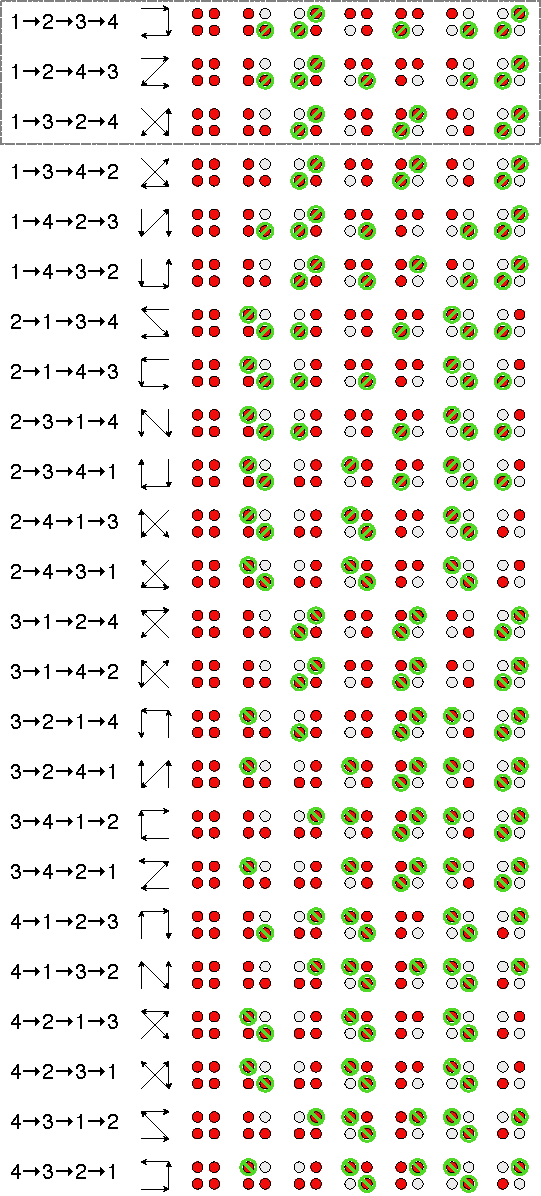
\includegraphics[width=0.3\textwidth]{Shortcuts}
	\caption{The catalog of all orderings of retesting a retest set
		of four points with points that logically can be left untested
		annotated. Observe that all orderings can be obtained from the first
		three by compositions of reflections and rotations. All orderings allow
		for either six or seven tests to be elided.}
	\label{fig:shortcuts}
\end{figure}


The rule for eliding tests in two dimensions can be stated as follows:
When a point tests negative, every point adjacent to that point
(excluding diagonals) must be positive and thus need not be tested.

TODO: Extend to $n$-dimensions. (The ``next'' dimension is a
``retest'' of the previous sample pooled tests but with pools instead of
individuals\ldots.)



\textbf{Fig. 7: Negative points in a three-dimensional retest set.}

TODO: Improvement on bounds of number of required tests.

\hypertarget{bounds-on-the-number-of-infected-individuals}{%
\section{Bounds on the number of infected
	individuals}\label{bounds-on-the-number-of-infected-individuals}}

The number of infected individuals can be estimated by stopping the
testing protocol after testing pools in the first $d$-dimensions,
eliding the retest phase.

\hypertarget{probabilistic-expectation-of-the-number-of-required-tests}{%
\section{Probabilistic expectation of the number of required
	tests}\label{probabilistic-expectation-of-the-number-of-required-tests}}

TODO.

\hspace{0pt} ---Include ``cutoff points'' of when scheme is no longer
advantageous. Should have its own section?

\hypertarget{summary}{%
\section{Summary}\label{summary}}

We assume the test for infection is perfect, i.e.~that the test is 100\%
effective and 100\% sensitive. The table below gives the definition of
the variables used.

\hypertarget{variables-used}{%
\subsection{Variables used}\label{variables-used}}

\begin{footnotesize}

\begin{longtable}[]{@{}llll@{}}
\toprule
\begin{minipage}[b]{0.08\columnwidth}\raggedright
	Variable\strut
\end{minipage} & \begin{minipage}[b]{0.28\columnwidth}\raggedright
	Meaning\strut
\end{minipage} & \begin{minipage}[b]{0.28\columnwidth}\raggedright
	Formula\strut
\end{minipage} & \begin{minipage}[b]{0.24\columnwidth}\raggedright
	How It's Determined\strut
\end{minipage}\tabularnewline
\midrule
\endhead
\begin{minipage}[t]{0.08\columnwidth}\raggedright
	$N$\strut
\end{minipage} & \begin{minipage}[t]{0.28\columnwidth}\raggedright
	Number of individuals in the population being tested\strut
\end{minipage} & \begin{minipage}[t]{0.28\columnwidth}\raggedright
	\strut
\end{minipage} & \begin{minipage}[t]{0.24\columnwidth}\raggedright
	Chosen\strut
\end{minipage}\tabularnewline
\begin{minipage}[t]{0.08\columnwidth}\raggedright
	$n$\strut
\end{minipage} & \begin{minipage}[t]{0.28\columnwidth}\raggedright
	Number of pools (one-dimensional pooling).\strut
\end{minipage} & \begin{minipage}[t]{0.28\columnwidth}\raggedright
	\strut
\end{minipage} & \begin{minipage}[t]{0.24\columnwidth}\raggedright
	Chosen\strut
\end{minipage}\tabularnewline
\begin{minipage}[t]{0.08\columnwidth}\raggedright
	$g$\strut
\end{minipage} & \begin{minipage}[t]{0.28\columnwidth}\raggedright
	Size of each pool (one-dimensional pooling)\strut
\end{minipage} & \begin{minipage}[t]{0.28\columnwidth}\raggedright
	$g:=N/n$\strut
\end{minipage} & \begin{minipage}[t]{0.24\columnwidth}\raggedright
	Derived from chosen values of $N$ and $n$\strut
\end{minipage}\tabularnewline
\begin{minipage}[t]{0.08\columnwidth}\raggedright
	$d$\strut
\end{minipage} & \begin{minipage}[t]{0.28\columnwidth}\raggedright
	Number of dimensions\strut
\end{minipage} & \begin{minipage}[t]{0.28\columnwidth}\raggedright
	\strut
\end{minipage} & \begin{minipage}[t]{0.24\columnwidth}\raggedright
	Chosen\strut
\end{minipage}\tabularnewline
\begin{minipage}[t]{0.08\columnwidth}\raggedright
	$g_j$\strut
\end{minipage} & \begin{minipage}[t]{0.28\columnwidth}\raggedright
	Size of each pool along dimension $j$, that is, in which the
	$j^\text{th}$ coordinate is constant. Each $g_j$ is an integer
	factor of $N$.\strut
\end{minipage} & \begin{minipage}[t]{0.28\columnwidth}\raggedright
	$N=\prod_{j=1}^d g_j$\strut
\end{minipage} & \begin{minipage}[t]{0.24\columnwidth}\raggedright
	Chosen\strut
\end{minipage}\tabularnewline
\begin{minipage}[t]{0.08\columnwidth}\raggedright
	$k$\strut
\end{minipage} & \begin{minipage}[t]{0.28\columnwidth}\raggedright
	Number of positive pools (one-dimensional pooling)\strut
\end{minipage} & \begin{minipage}[t]{0.28\columnwidth}\raggedright
	\strut
\end{minipage} & \begin{minipage}[t]{0.24\columnwidth}\raggedright
	Empirically\strut
\end{minipage}\tabularnewline
\begin{minipage}[t]{0.08\columnwidth}\raggedright
	$k_j$\strut
\end{minipage} & \begin{minipage}[t]{0.28\columnwidth}\raggedright
	Number of positive pools among the total number of pools $g_j$ along
	dimension $j$\strut
\end{minipage} & \begin{minipage}[t]{0.28\columnwidth}\raggedright
	\strut
\end{minipage} & \begin{minipage}[t]{0.24\columnwidth}\raggedright
	Empirically\strut
\end{minipage}\tabularnewline
\begin{minipage}[t]{0.08\columnwidth}\raggedright
	$i$\strut
\end{minipage} & \begin{minipage}[t]{0.28\columnwidth}\raggedright
	Number of infected individuals within the population\strut
\end{minipage} & \begin{minipage}[t]{0.28\columnwidth}\raggedright
	\strut
\end{minipage} & \begin{minipage}[t]{0.24\columnwidth}\raggedright
	Empirically\strut
\end{minipage}\tabularnewline
\begin{minipage}[t]{0.08\columnwidth}\raggedright
	$T$\strut
\end{minipage} & \begin{minipage}[t]{0.28\columnwidth}\raggedright
	Number of tests required for the given application of the testing
	protocol\strut
\end{minipage} & \begin{minipage}[t]{0.28\columnwidth}\raggedright
	$T= \sum_{j=1}^d g_j + \prod_{j=1}^d k_j$\strut
\end{minipage} & \begin{minipage}[t]{0.24\columnwidth}\raggedright
	Chosen\strut
\end{minipage}\tabularnewline
\begin{minipage}[t]{0.08\columnwidth}\raggedright
	$T_{\text{max}}$\strut
\end{minipage} & \begin{minipage}[t]{0.28\columnwidth}\raggedright
	Maximum number of tests that can be required for the given testing
	protocol\strut
\end{minipage} & \begin{minipage}[t]{0.28\columnwidth}\raggedright
	$T_{\text{max}}=\begin{cases} \sum_{j=1}^d g_j + i^d& i<g_j \forall j \\ \sum_{j=1}^d g_j + N & i=N\\ \sum_{j=1}^d g_j + \prod_{j=1}^d \text{min}(i, g_j) & \text{generally} \end{cases}$\strut
\end{minipage} & \begin{minipage}[t]{0.24\columnwidth}\raggedright
	Derived from test design and empirical value of $i$\strut
\end{minipage}\tabularnewline
\begin{minipage}[t]{0.08\columnwidth}\raggedright
	$T_{\text{min}}$\strut
\end{minipage} & \begin{minipage}[t]{0.28\columnwidth}\raggedright
	Minimum number of tests that can be required for the given testing
	protocol\strut
\end{minipage} & \begin{minipage}[t]{0.28\columnwidth}\raggedright
	$T_{\text{min}}=\text{min}_j \;(g_j)$\strut
\end{minipage} & \begin{minipage}[t]{0.24\columnwidth}\raggedright
	Derived from chosen values of $N$ and $n$\strut
\end{minipage}\tabularnewline
\begin{minipage}[t]{0.08\columnwidth}\raggedright
	\strut
\end{minipage} & \begin{minipage}[t]{0.28\columnwidth}\raggedright
	\strut
\end{minipage} & \begin{minipage}[t]{0.28\columnwidth}\raggedright
	\strut
\end{minipage} & \begin{minipage}[t]{0.24\columnwidth}\raggedright
	\strut
\end{minipage}\tabularnewline
\bottomrule
\end{longtable}


\end{footnotesize}


\hypertarget{theorems}{%
\subsection{Theorems}\label{theorems}}

\begin{enumerate}
\def\labelenumi{\arabic{enumi}.}
\item
The total number of tests required for $d$-dimensional pooling is
\[
T_{\text{max}}=\sum_{j=1}^d g_j + \prod_{j=1}^d \text{min}(i, g_j) =
\begin{cases} 
\sum_{j=1}^d g_j + i^d& \text{if }i<g_j\; \forall j \\ 
\sum_{j=1}^d g_j + N & \text{if }i=N 
\end{cases}.
\]
\item
As a consequence of (1), pooled sample testing is of greatest benefit
when the number of infected individuals is small (close to 0).
\item
As a consequence of (1), pooled sample testing requires more tests
than naive sample testing if the number of infected individuals is
large (close to $N$).
\item
Dimensions must be tested in order from smallest to largest to detect
the absence of infected individuals after $\text{min}_j \;g_j$
tests, which is optimal.
\item
The number of tests used on pools is the total number of pools, which
is $\sum_{j=1}^d g_j$.
\item
The number of retests of individuals required is
\[
\prod_{j=1}^d \text{min}(i, g_j) = 
\begin{cases} 
i^d& \text{if }i<g_j\;\forall j \\
N & \text{if }i=N \end{cases}.\]
\end{enumerate}


\section*{Acknowledgment}
Thanks to Andy Rhyne for encouragement, fruitful discussions, and valuable feedback.
All errors are my own.

\end{document}
